\documentclass[11pt, oneside]{article}   	% use "amsart" instead of "article" for AMSLaTeX format
\usepackage{geometry}                		% See geometry.pdf to learn the layout options. There are lots.
\geometry{letterpaper}                   		% ... or a4paper or a5paper or ... 
%\geometry{landscape}                		% Activate for for rotated page geometry
%\usepackage[parfill]{parskip}    		% Activate to begin paragraphs with an empty line rather than an indent
\usepackage{graphicx}				% Use pdf, png, jpg, or eps§ with pdflatex; use eps in DVI mode
\usepackage{tikz}
\usetikzlibrary{arrows}								% TeX will automatically convert eps --> pdf in pdflatex		
\usepackage{amssymb}

\title{Graph}
\author{Bohan Xu}
%\date{}							% Activate to display a given date or no date

\begin{document}
\maketitle
\section{question 2}

initial graph

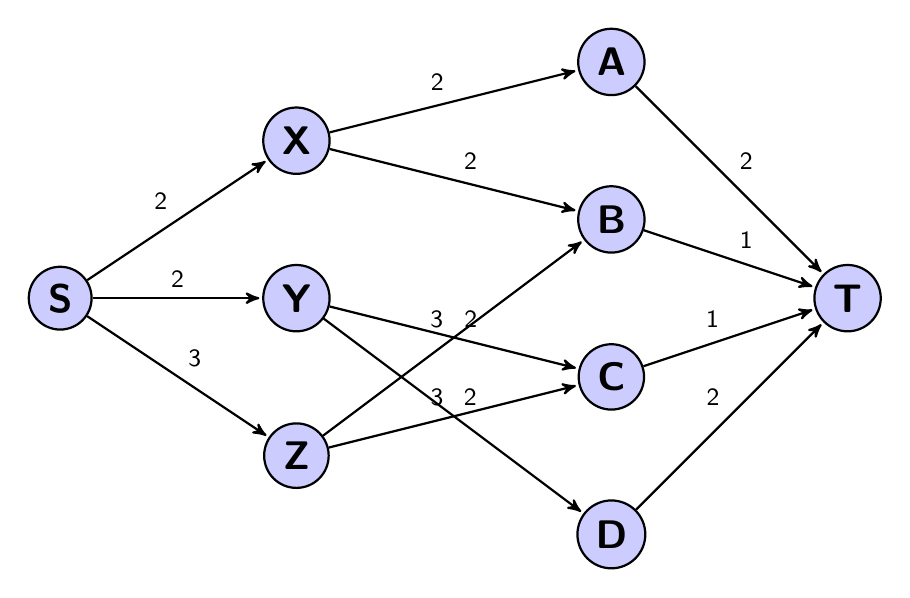
\begin{tikzpicture}[->,>=stealth',shorten >=1pt,auto,node distance=3cm,
  thick,main node/.style={circle,fill=blue!20,draw,font=\sffamily\Large\bfseries}]

  \node[main node]  (1) at (5,5) {S};
  \node[main node]  (2) at (8, 7) {X};
  \node[main node]  (3) at (8, 5) {Y};
  \node[main node]  (4) at (8, 3) {Z};
  \node[main node]  (5) at (12, 8) {A};
  \node[main node]  (6) at (12, 6) {B};
  \node[main node]  (7) at (12, 4) {C};
  \node[main node]  (8) at (12, 2) {D};    
  \node[main node]  (9) at (15, 5) {T};
  
  \path[every node/.style={font=\sffamily\small}]
    (1) edge node {2} (2)
    (1) edge node  {2} (3)
    (1) edge node  {3} (4)
    (2) edge node  {2} (5)
    (2) edge node  {2} (6)
    (3) edge node  {2} (7)
    (3) edge node  {2} (8)
    (4) edge node  {3} (6)
    (4) edge node  {3} (7)
    (5) edge node  {2} (9)
    (6) edge node  {1} (9)
    (7) edge node  {1} (9)
    (8) edge node  {2} (9);
    
\end{tikzpicture}

\clearpage
%2
path: 1-2-5-9

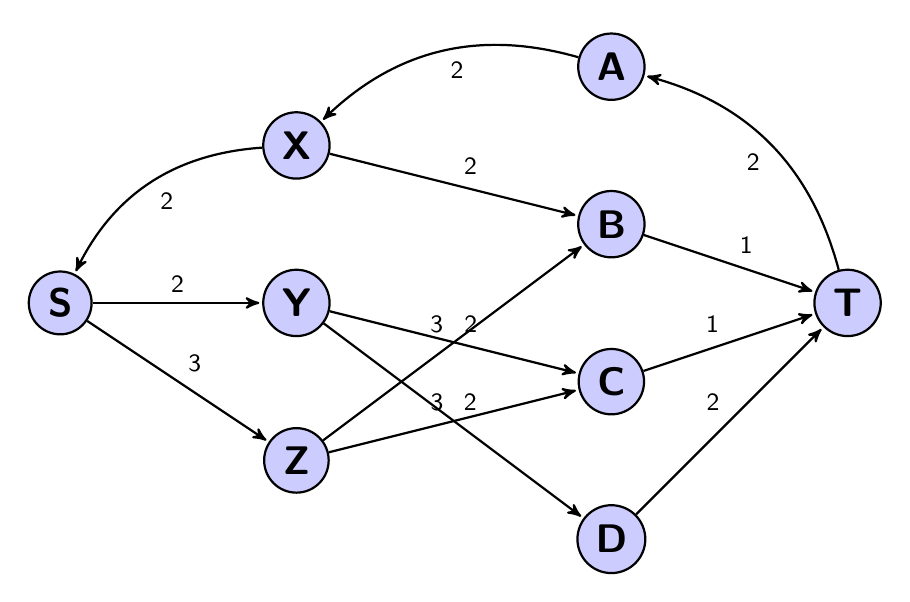
\begin{tikzpicture}[->,>=stealth',shorten >=1pt,auto,node distance=3cm,
  thick,main node/.style={circle,fill=blue!20,draw,font=\sffamily\Large\bfseries}]

  \node[main node]  (1) at (5,5) {S};
  \node[main node]  (2) at (8, 7) {X};
  \node[main node]  (3) at (8, 5) {Y};
  \node[main node]  (4) at (8, 3) {Z};
  \node[main node]  (5) at (12, 8) {A};
  \node[main node]  (6) at (12, 6) {B};
  \node[main node]  (7) at (12, 4) {C};
  \node[main node]  (8) at (12, 2) {D};    
  \node[main node]  (9) at (15, 5) {T};
  
  \path[every node/.style={font=\sffamily\small}]
    (1) edge node  {2} (3)
    (1) edge node  {3} (4)
    (2) edge node  {2} (6)
    (3) edge node  {2} (7)
    (3) edge node  {2} (8)
    (4) edge node  {3} (6)
    (4) edge node  {3} (7)
    (6) edge node  {1} (9)
    (7) edge node  {1} (9)
    (8) edge node  {2} (9)
    %add back edges
    (2) edge [bend right] node {2} (1)
    (5) edge [bend right] node  {2} (2)
    (9) edge [bend right] node  {2} (5);
    
\end{tikzpicture}

\-
\\
\\
path: 1 3 7 9

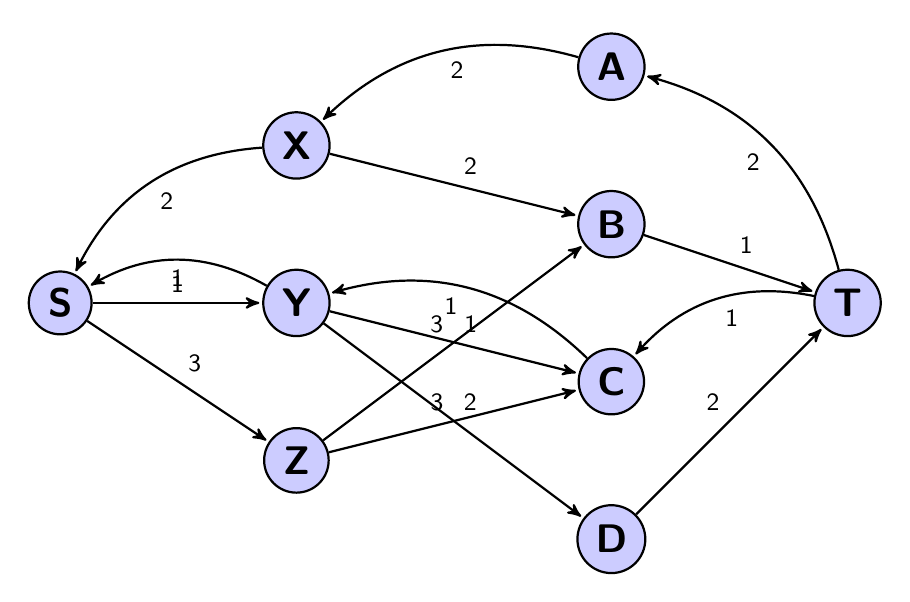
\begin{tikzpicture}[->,>=stealth',shorten >=1pt,auto,node distance=3cm,
  thick,main node/.style={circle,fill=blue!20,draw,font=\sffamily\Large\bfseries}]

  \node[main node]  (1) at (5,5) {S};
  \node[main node]  (2) at (8, 7) {X};
  \node[main node]  (3) at (8, 5) {Y};
  \node[main node]  (4) at (8, 3) {Z};
  \node[main node]  (5) at (12, 8) {A};
  \node[main node]  (6) at (12, 6) {B};
  \node[main node]  (7) at (12, 4) {C};
  \node[main node]  (8) at (12, 2) {D};    
  \node[main node]  (9) at (15, 5) {T};
  
  \path[every node/.style={font=\sffamily\small}]
%    (1) edge node  {2} (3)
    (1) edge node  {1} (3)
    (1) edge node  {3} (4)
    (2) edge node  {2} (6)
%    (3) edge node  {2} (7)
    (3) edge node  {1} (7)
    (3) edge node  {2} (8)
    (4) edge node  {3} (6)
    (4) edge node  {3} (7)
    (6) edge node  {1} (9)
% (7) edge node  {1} (9)
    (8) edge node  {2} (9)
    %add back edges
    (2) edge [bend right] node {2} (1)
    (5) edge [bend right] node  {2} (2)
    (9) edge [bend right] node  {2} (5)
    (3) edge [bend right] node  {1} (1)
    (7) edge [bend right] node  {1} (3)
    (9) edge [bend right] node  {1} (7);
    
\end{tikzpicture}

\clearpage
path: 1 3 8 9

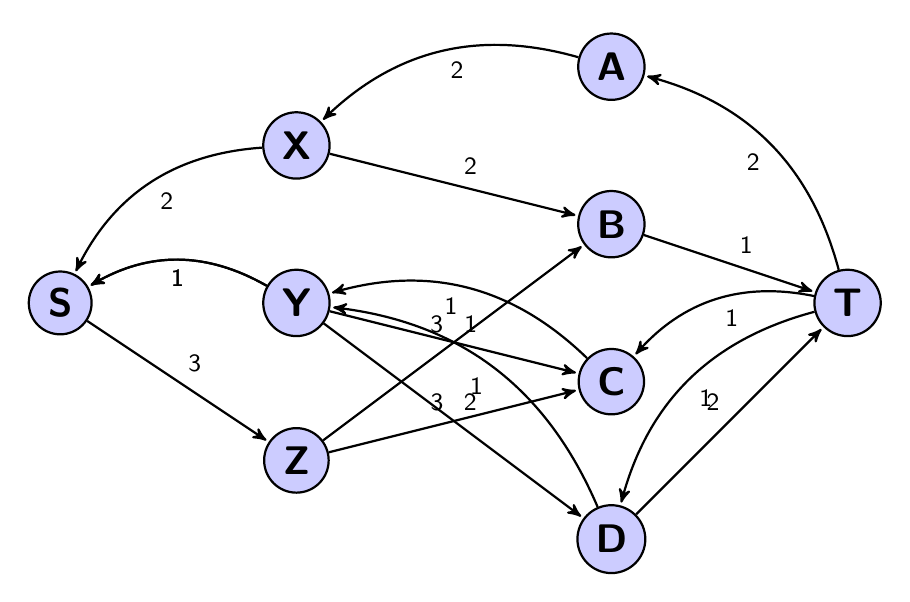
\begin{tikzpicture}[->,>=stealth',shorten >=1pt,auto,node distance=3cm,
  thick,main node/.style={circle,fill=blue!20,draw,font=\sffamily\Large\bfseries}]

  \node[main node]  (1) at (5,5) {S};
  \node[main node]  (2) at (8, 7) {X};
  \node[main node]  (3) at (8, 5) {Y};
  \node[main node]  (4) at (8, 3) {Z};
  \node[main node]  (5) at (12, 8) {A};
  \node[main node]  (6) at (12, 6) {B};
  \node[main node]  (7) at (12, 4) {C};
  \node[main node]  (8) at (12, 2) {D};    
  \node[main node]  (9) at (15, 5) {T};
  
  \path[every node/.style={font=\sffamily\small}]
    %(1) edge node  {1} (3)
    (1) edge node  {3} (4)
    (2) edge node  {2} (6)
    (3) edge node  {1} (7)
%    (3) edge node  {2} (8)
    (3) edge node  {2} (8)
    (4) edge node  {3} (6)
    (4) edge node  {3} (7)
    (6) edge node  {1} (9)
%    (8) edge node  {2} (9)
    (8) edge node  {2} (9)
    %add back edges
    (2) edge [bend right] node {2} (1)
    (5) edge [bend right] node  {2} (2)
    (9) edge [bend right] node  {2} (5)
    (3) edge [bend right] node  {1} (1)
    (7) edge [bend right] node  {1} (3)
    (9) edge [bend right] node  {1} (7)
    (3) edge [bend right] node  {1} (1)
    (8) edge [bend right] node  {1} (3)
    (9) edge [bend right] node  {1} (8);
    
    
\end{tikzpicture}

\-
\\
\\

path: 1 4 6 9 

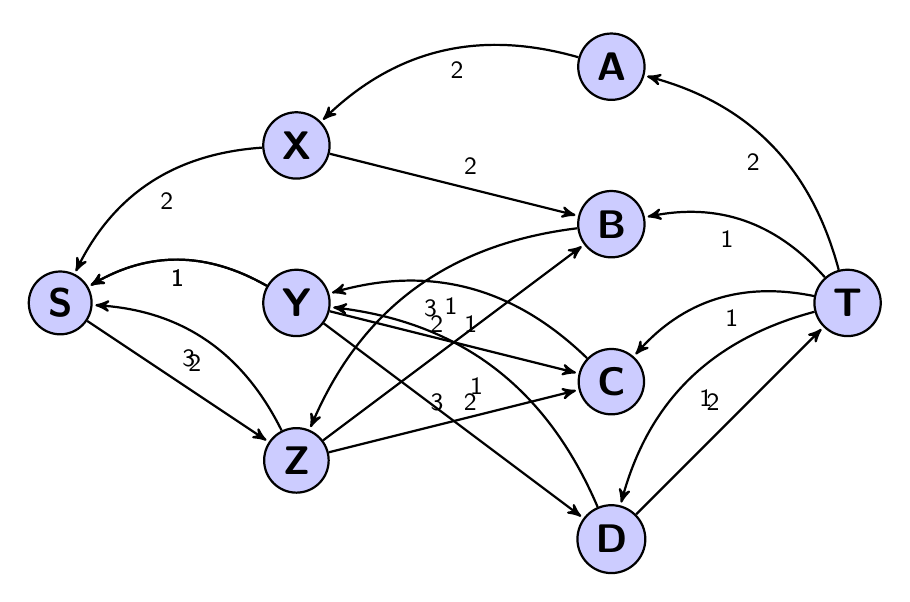
\begin{tikzpicture}[->,>=stealth',shorten >=1pt,auto,node distance=3cm,
  thick,main node/.style={circle,fill=blue!20,draw,font=\sffamily\Large\bfseries}]

  \node[main node]  (1) at (5,5) {S};
  \node[main node]  (2) at (8, 7) {X};
  \node[main node]  (3) at (8, 5) {Y};
  \node[main node]  (4) at (8, 3) {Z};
  \node[main node]  (5) at (12, 8) {A};
  \node[main node]  (6) at (12, 6) {B};
  \node[main node]  (7) at (12, 4) {C};
  \node[main node]  (8) at (12, 2) {D};    
  \node[main node]  (9) at (15, 5) {T};
  
  \path[every node/.style={font=\sffamily\small}]
%    (1) edge node  {3} (4)
    (1) edge node  {2} (4)
    (2) edge node  {2} (6)
    (3) edge node  {1} (7)
    (3) edge node  {2} (8)
%    (4) edge node  {3} (6)
    (4) edge node  {2} (6)
    (4) edge node  {3} (7)
%    (6) edge node  {1} (9)
    (8) edge node  {2} (9)
    %add back edges
    (2) edge [bend right] node {2} (1)
    (5) edge [bend right] node  {2} (2)
    (9) edge [bend right] node  {2} (5)
    (3) edge [bend right] node  {1} (1)
    (7) edge [bend right] node  {1} (3)
    (9) edge [bend right] node  {1} (7)
    (3) edge [bend right] node  {1} (1)
    (8) edge [bend right] node  {1} (3)
    (9) edge [bend right] node  {1} (8)
    (4) edge [bend right] node  {3} (1)
    (6) edge [bend right] node  {3} (4)
    (9) edge [bend right] node  {1} (6);
\end{tikzpicture}

\clearpage

path: 1 4 7 3 8 9 

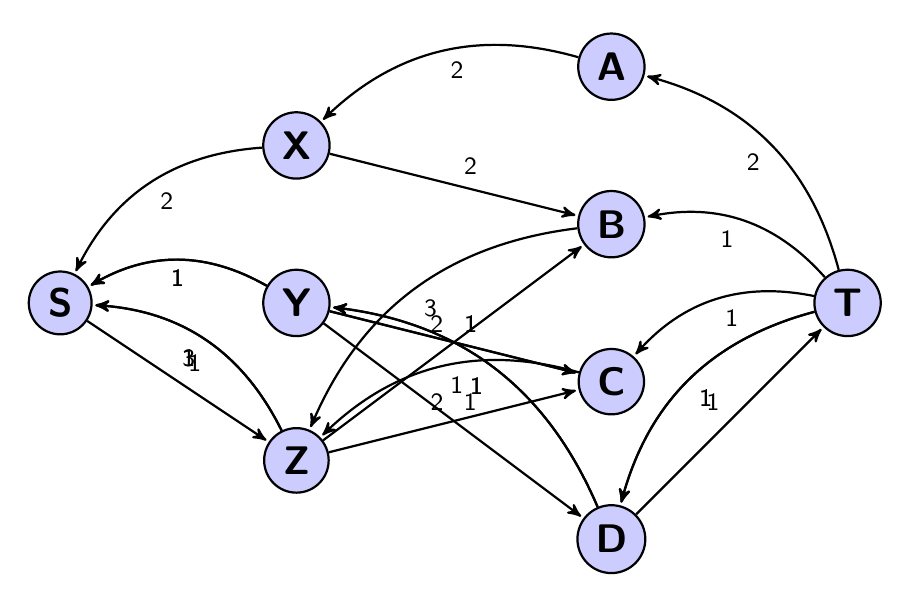
\begin{tikzpicture}[->,>=stealth',shorten >=1pt,auto,node distance=3cm,
  thick,main node/.style={circle,fill=blue!20,draw,font=\sffamily\Large\bfseries}]

  \node[main node]  (1) at (5,5) {S};
  \node[main node]  (2) at (8, 7) {X};
  \node[main node]  (3) at (8, 5) {Y};
  \node[main node]  (4) at (8, 3) {Z};
  \node[main node]  (5) at (12, 8) {A};
  \node[main node]  (6) at (12, 6) {B};
  \node[main node]  (7) at (12, 4) {C};
  \node[main node]  (8) at (12, 2) {D};    
  \node[main node]  (9) at (15, 5) {T};
  
  \path[every node/.style={font=\sffamily\small}]
 %   (1) edge node  {2} (4)
    (1) edge node  {1} (4)
    (2) edge node  {2} (6)
    (3) edge node  {1} (7)
%    (3) edge node  {2} (8)
    (3) edge node  {1} (8)
    (4) edge node  {2} (6)
%    (4) edge node  {3} (7)
    (4) edge node  {2} (7)
%    (8) edge node  {2} (9)
    (8) edge node  {1} (9)
    % back back edge
    (3) edge node  {1} (7)
    %add back edges
    (2) edge [bend right] node {2} (1)
    (5) edge [bend right] node  {2} (2)
    (9) edge [bend right] node  {2} (5)
    (3) edge [bend right] node  {1} (1)
%    (7) edge [bend right] node  {1} (3)
    (9) edge [bend right] node  {1} (7)
    (3) edge [bend right] node  {1} (1)
    (8) edge [bend right] node  {1} (3)
    (9) edge [bend right] node  {1} (8)
    (4) edge [bend right] node  {3} (1)
    (6) edge [bend right] node  {3} (4)
    (9) edge [bend right] node  {1} (6)   
    (4) edge [bend right] node  {1} (1)
    (8) edge [bend right] node  {1} (3)
    (7) edge [bend right] node  {1} (4)
    (9) edge [bend right] node  {1} (8);
    
    
    
\end{tikzpicture}

%%%%%%%%%%%%%%%%%%%%%%%%%%%%%%%%%%%%%%%%%%%%%%%%%

\clearpage

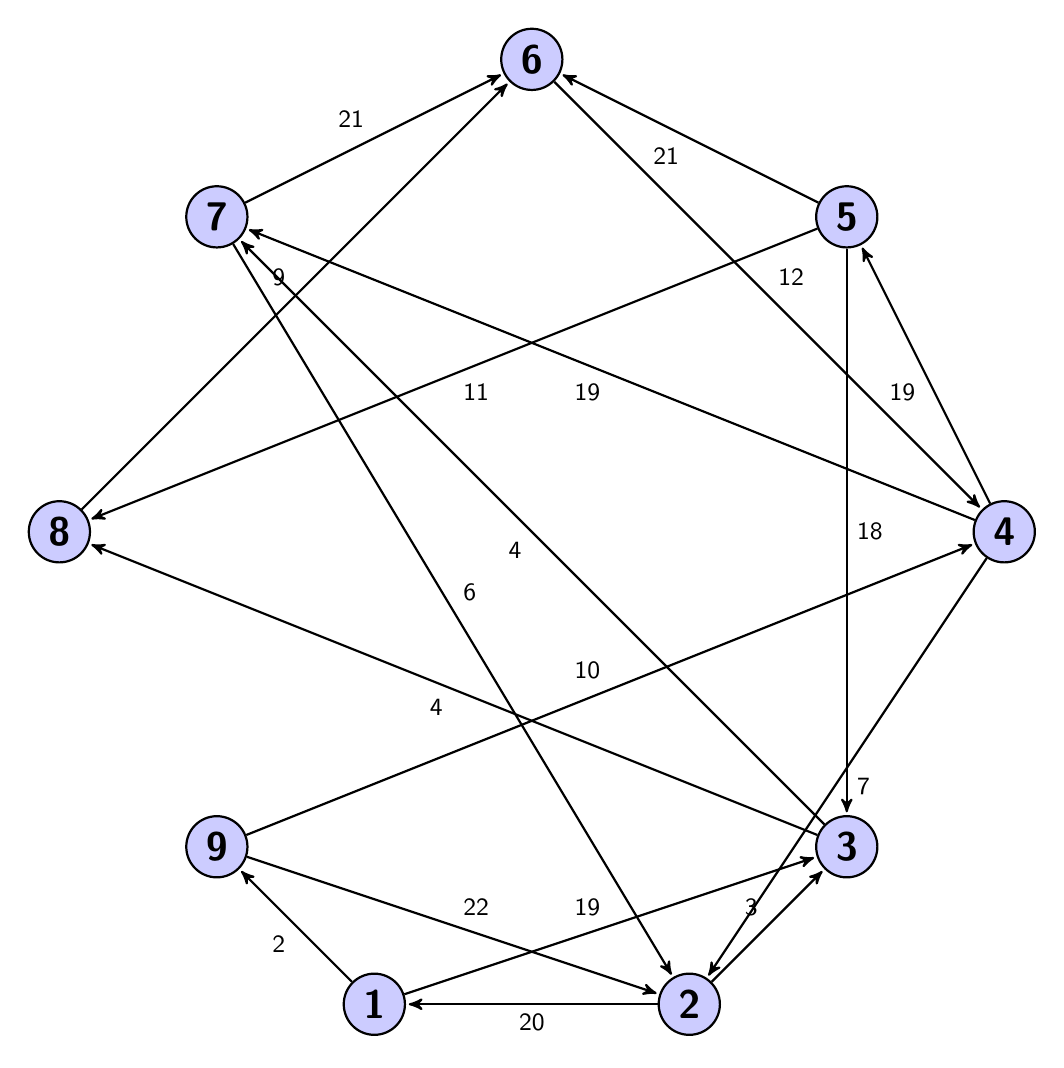
\begin{tikzpicture}[->,>=stealth',shorten >=1pt,auto,node distance=3cm,thick,main node/.style={circle,fill=blue!20,draw,font=\sffamily\Large\bfseries}]
  \node[main node] (1) at (10,0) {1};
  \node[main node] (2) at (14,0) {2};
  \node[main node] (3) at (16,2) {3};
  \node[main node] (4) at (18,6) {4};
  \node[main node] (5) at (16,10) {5};
  \node[main node] (6) at (12,12) {6};
  \node[main node] (7) at (8,10) {7};
  \node[main node] (8) at (6,6) {8};
  \node[main node] (9) at (8,2) {9};

\path[every node/.style={font=\sffamily\small}]
  (1) edge node {19} (3)
  (1) edge node {2} (9)
  (2) edge node {20} (1)
  (2) edge node {3} (3)
  (3) edge node {4} (7)
  (3) edge node {4} (8)
  (4) edge node {7} (2)
  (4) edge node {19} (5)
  (4) edge node {19} (7)
  (5) edge node {18} (3)
  (5) edge node {21} (6)
  (5) edge node {11} (8)
  (6) edge node {12} (4)
  (7) edge node {6} (2)
  (7) edge node {21} (6)
  (8) edge node {9} (6)
  (9) edge node {22} (2)
  (9) edge node {10} (4)
;
\end{tikzpicture}

\clearpage
path:5 3 7 2 
\\
capacity:4

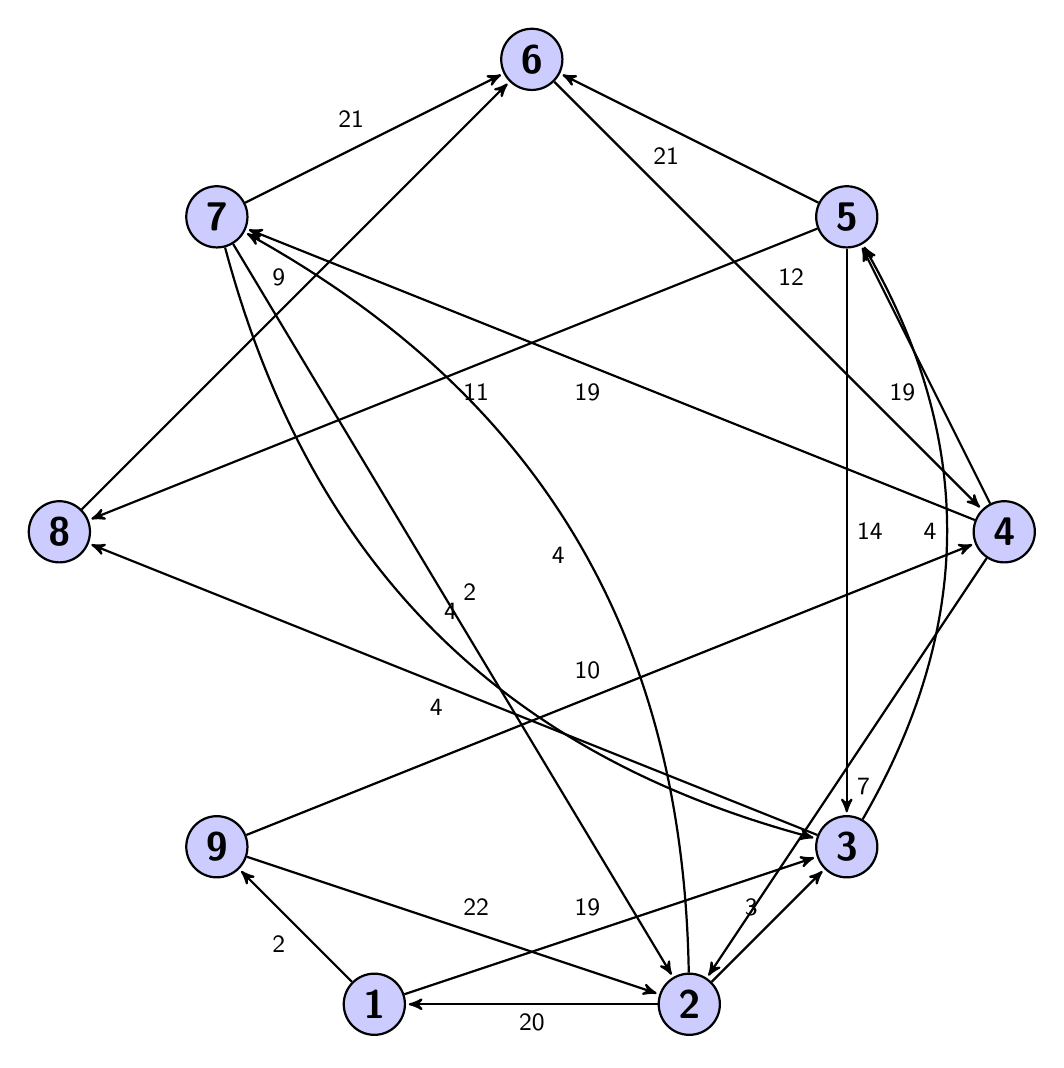
\begin{tikzpicture}[->,>=stealth',shorten >=1pt,auto,node distance=3cm,thick,main node/.style={circle,fill=blue!20,draw,font=\sffamily\Large\bfseries}]
  \node[main node] (1) at (10,0) {1};
  \node[main node] (2) at (14,0) {2};
  \node[main node] (3) at (16,2) {3};
  \node[main node] (4) at (18,6) {4};
  \node[main node] (5) at (16,10) {5};
  \node[main node] (6) at (12,12) {6};
  \node[main node] (7) at (8,10) {7};
  \node[main node] (8) at (6,6) {8};
  \node[main node] (9) at (8,2) {9};

\path[every node/.style={font=\sffamily\small}]
  (1) edge node {19} (3)
  (1) edge node {2} (9)
  (2) edge node {20} (1)
  (2) edge node {3} (3)
  (3) edge node {4} (8)
  (4) edge node {7} (2)
  (4) edge node {19} (5)
  (4) edge node {19} (7)
  (5) edge node {14} (3)
  (5) edge node {21} (6)
  (5) edge node {11} (8)
  (6) edge node {12} (4)
  (7) edge node {2} (2)
  (7) edge node {21} (6)
  (8) edge node {9} (6)
  (9) edge node {22} (2)
  (9) edge node {10} (4)
  (3) edge [bend right] node  {4} (5)
  (2) edge [bend right] node  {4} (7)
  (7) edge [bend right] node  {4} (3)
;
\end{tikzpicture}

\clearpage
path:5 6 4 2 
\\
capacity:7

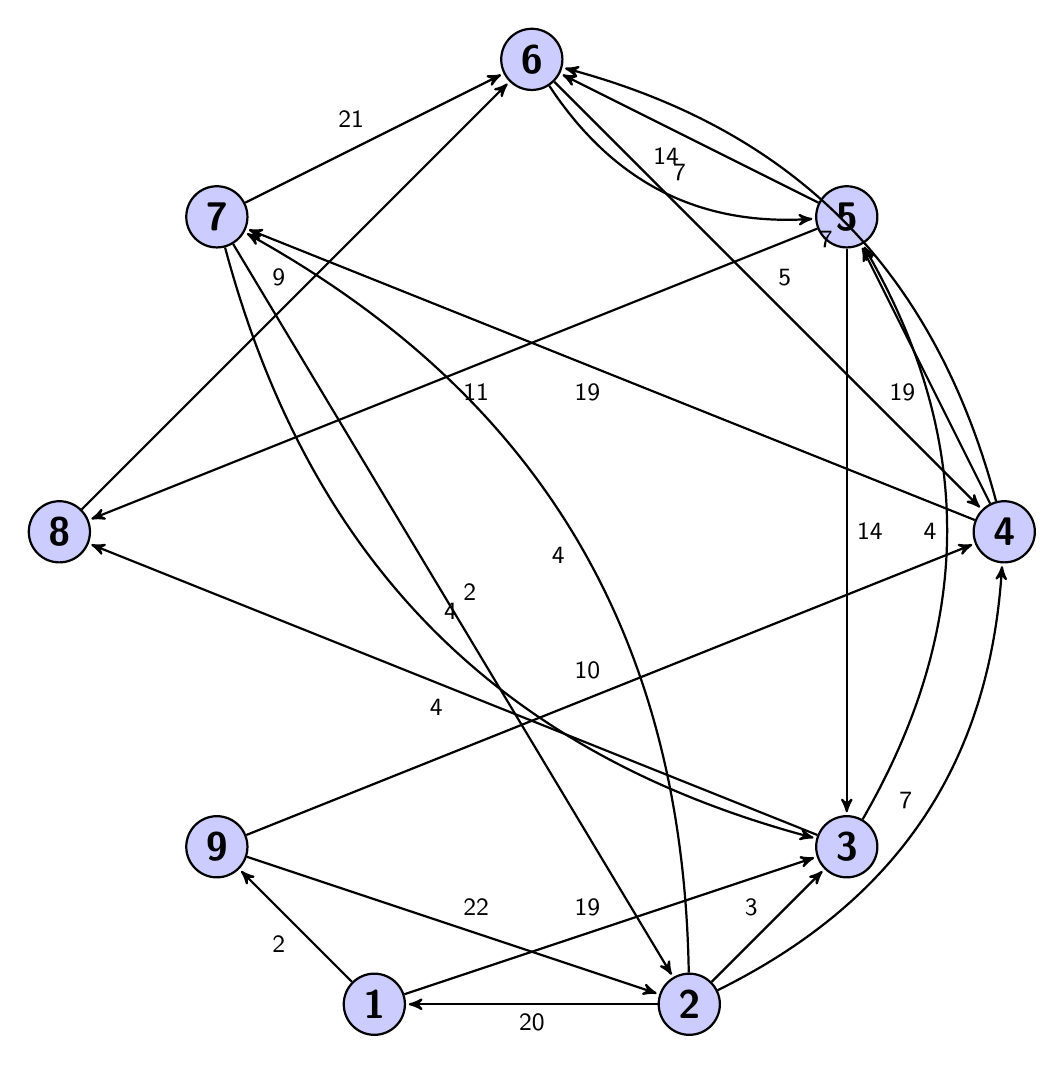
\begin{tikzpicture}[->,>=stealth',shorten >=1pt,auto,node distance=3cm,thick,main node/.style={circle,fill=blue!20,draw,font=\sffamily\Large\bfseries}]
  \node[main node] (1) at (10,0) {1};
  \node[main node] (2) at (14,0) {2};
  \node[main node] (3) at (16,2) {3};
  \node[main node] (4) at (18,6) {4};
  \node[main node] (5) at (16,10) {5};
  \node[main node] (6) at (12,12) {6};
  \node[main node] (7) at (8,10) {7};
  \node[main node] (8) at (6,6) {8};
  \node[main node] (9) at (8,2) {9};

\path[every node/.style={font=\sffamily\small}]
  (1) edge node {19} (3)
  (1) edge node {2} (9)
  (2) edge node {20} (1)
  (2) edge node {3} (3)
  (3) edge node {4} (8)
  (4) edge node {19} (5)
  (4) edge node {19} (7)
  (5) edge node {14} (3)
  (5) edge node {14} (6)
  (5) edge node {11} (8)
  (6) edge node {5} (4)
  (7) edge node {2} (2)
  (7) edge node {21} (6)
  (8) edge node {9} (6)
  (9) edge node {22} (2)
  (9) edge node {10} (4)
  (2) edge [bend right] node  {7} (4)
  (3) edge [bend right] node  {4} (5)
  (2) edge [bend right] node  {4} (7)
  (7) edge [bend right] node  {4} (3)
  (6) edge [bend right] node  {7} (5)
  (4) edge [bend right] node  {7} (6)
;
\end{tikzpicture}

\clearpage
path:5 6 4 7 2 
\\
capacity:2

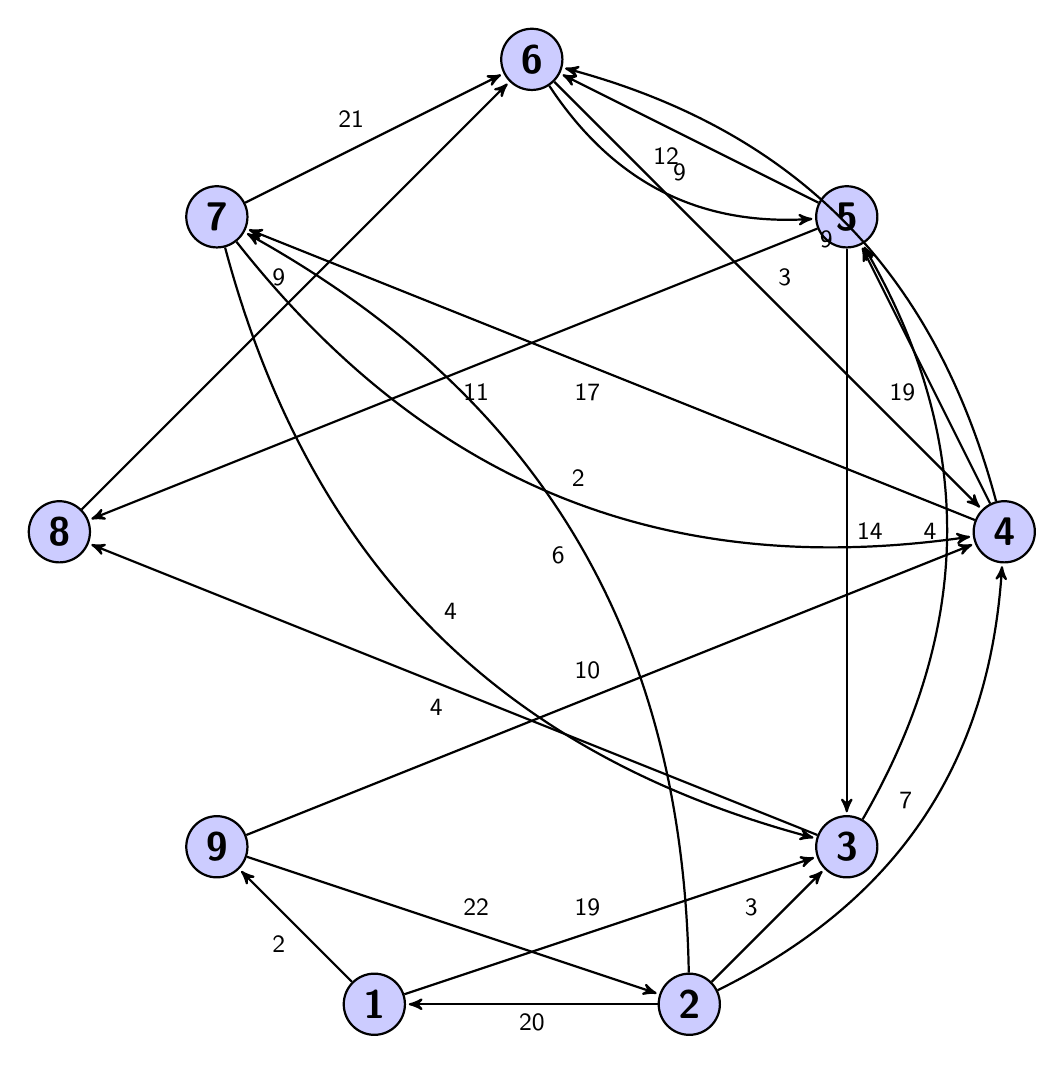
\begin{tikzpicture}[->,>=stealth',shorten >=1pt,auto,node distance=3cm,thick,main node/.style={circle,fill=blue!20,draw,font=\sffamily\Large\bfseries}]
  \node[main node] (1) at (10,0) {1};
  \node[main node] (2) at (14,0) {2};
  \node[main node] (3) at (16,2) {3};
  \node[main node] (4) at (18,6) {4};
  \node[main node] (5) at (16,10) {5};
  \node[main node] (6) at (12,12) {6};
  \node[main node] (7) at (8,10) {7};
  \node[main node] (8) at (6,6) {8};
  \node[main node] (9) at (8,2) {9};

\path[every node/.style={font=\sffamily\small}]
  (1) edge node {19} (3)
  (1) edge node {2} (9)
  (2) edge node {20} (1)
  (2) edge node {3} (3)
  (3) edge node {4} (8)
  (4) edge node {19} (5)
  (4) edge node {17} (7)
  (5) edge node {14} (3)
  (5) edge node {12} (6)
  (5) edge node {11} (8)
  (6) edge node {3} (4)
  (7) edge node {21} (6)
  (8) edge node {9} (6)
  (9) edge node {22} (2)
  (9) edge node {10} (4)
  (2) edge [bend right] node  {7} (4)
  (3) edge [bend right] node  {4} (5)
  (2) edge [bend right] node  {6} (7)
  (7) edge [bend right] node  {4} (3)
  (6) edge [bend right] node  {9} (5)
  (4) edge [bend right] node  {9} (6)
  (7) edge [bend right] node  {2} (4)
;
\end{tikzpicture}

13


%%%%%%%%%%%%%%%%%%%%%%%%%%%%%%%%%%%%%%%%%%%%%%%%%


\clearpage

\section{with process}


 \clearpage

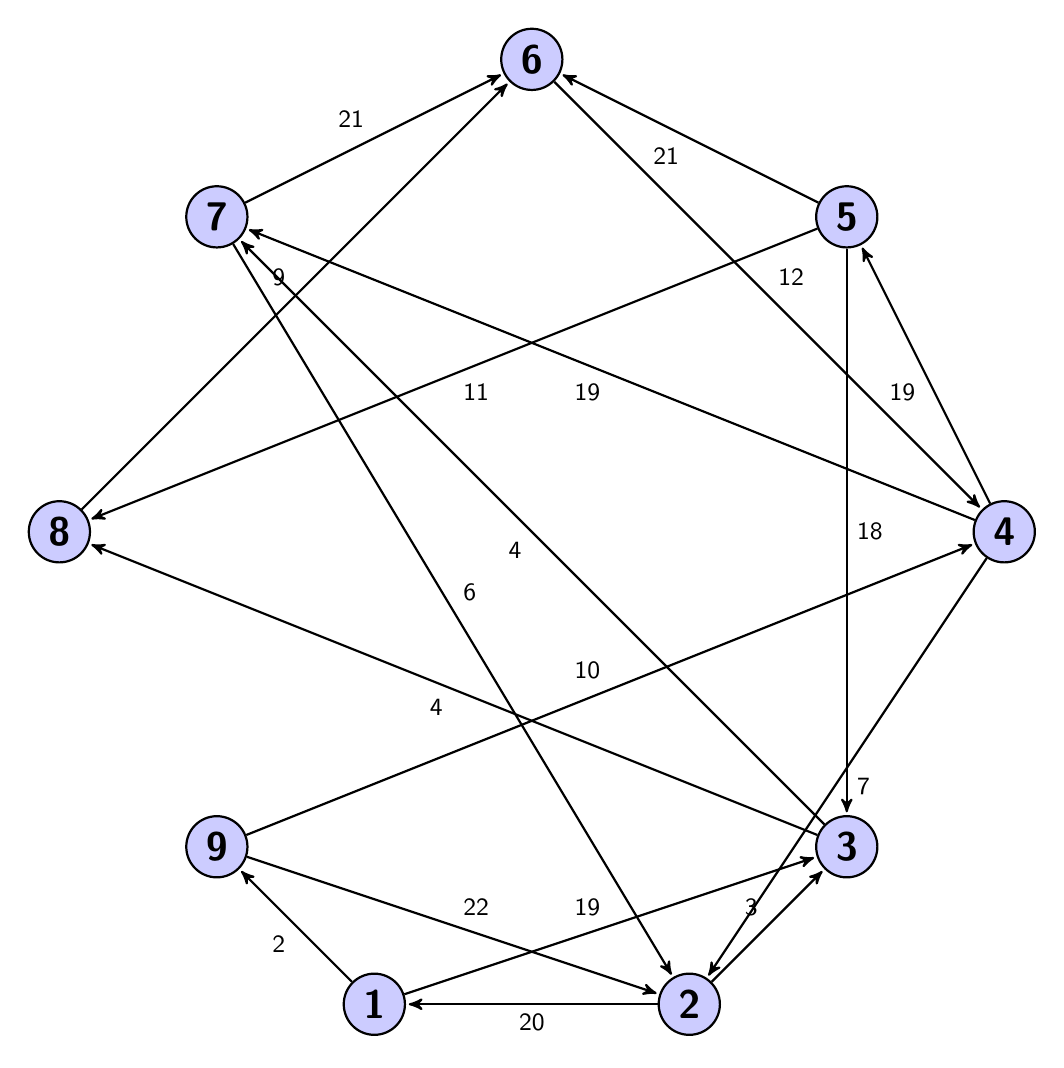
\begin{tikzpicture}[->,>=stealth',shorten >=1pt,auto,node distance=3cm,thick,main node/.style={circle,fill=blue!20,draw,font=\sffamily\Large\bfseries}]
  \node[main node] (1) at (10,0) {1};
  \node[main node] (2) at (14,0) {2};
  \node[main node] (3) at (16,2) {3};
  \node[main node] (4) at (18,6) {4};
  \node[main node] (5) at (16,10) {5};
  \node[main node] (6) at (12,12) {6};
  \node[main node] (7) at (8,10) {7};
  \node[main node] (8) at (6,6) {8};
  \node[main node] (9) at (8,2) {9};

\path[every node/.style={font=\sffamily\small}]
  (1) edge node {19} (3)
  (1) edge node {2} (9)
  (2) edge node {20} (1)
  (2) edge node {3} (3)
  (3) edge node {4} (7)
  (3) edge node {4} (8)
  (4) edge node {7} (2)
  (4) edge node {19} (5)
  (4) edge node {19} (7)
  (5) edge node {18} (3)
  (5) edge node {21} (6)
  (5) edge node {11} (8)
  (6) edge node {12} (4)
  (7) edge node {6} (2)
  (7) edge node {21} (6)
  (8) edge node {9} (6)
  (9) edge node {22} (2)
  (9) edge node {10} (4)
;
\end{tikzpicture}


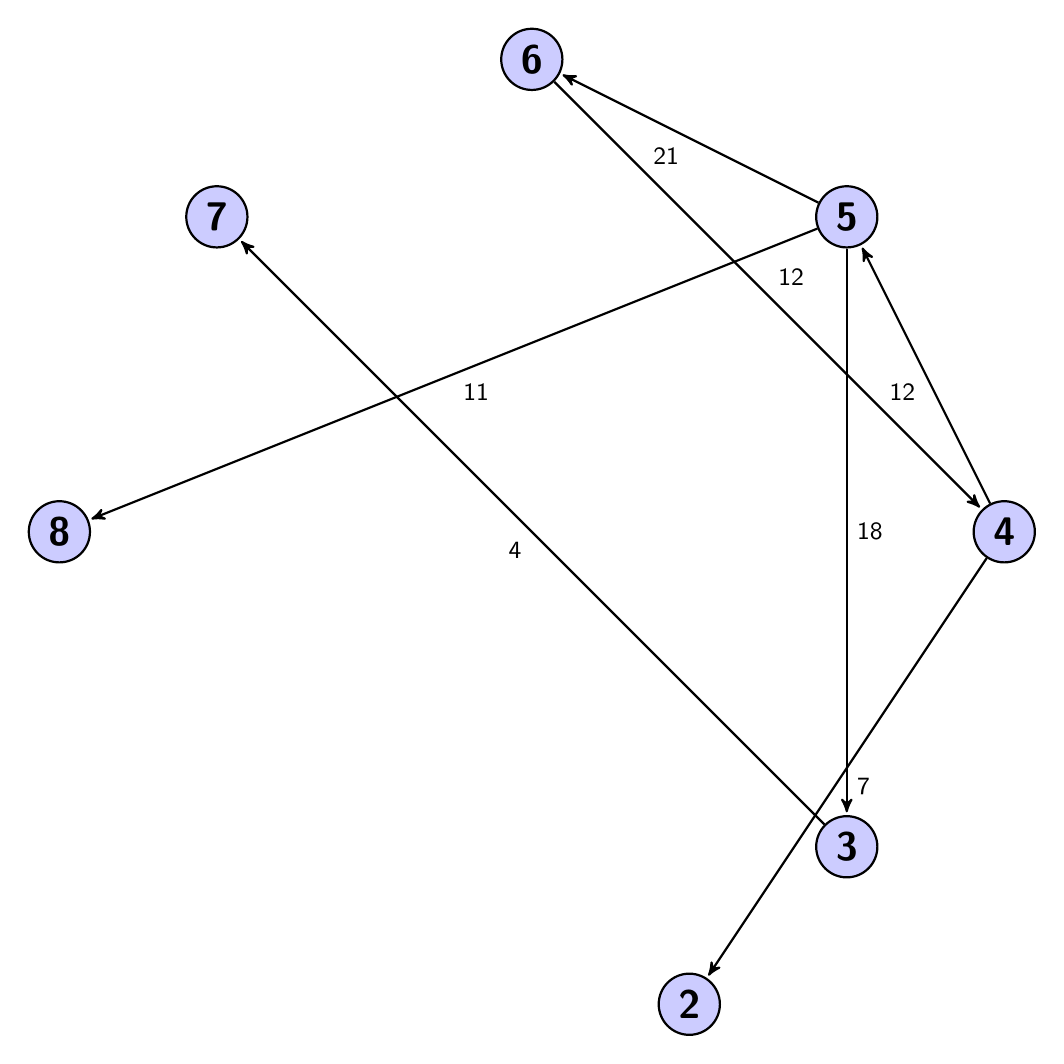
\begin{tikzpicture}[->,>=stealth',shorten >=1pt,auto,node distance=3cm,thick,main node/.style={circle,fill=blue!20,draw,font=\sffamily\Large\bfseries}]
  \node[main node] (2) at (14,0) {2};
  \node[main node] (3) at (16,2) {3};
  \node[main node] (4) at (18,6) {4};
  \node[main node] (5) at (16,10) {5};
  \node[main node] (6) at (12,12) {6};
  \node[main node] (7) at (8,10) {7};
  \node[main node] (8) at (6,6) {8};

\path[every node/.style={font=\sffamily\small}]
  (4) edge node {7} (2)
  (5) edge node {18} (3)
  (6) edge node {12} (4)
  (4) edge node {12} (5)
  (5) edge node {21} (6)
  (3) edge node {4} (7)
  (5) edge node {11} (8)
;
\end{tikzpicture}

\clearpage
path:5 6 4 2 
\\
capacity:7

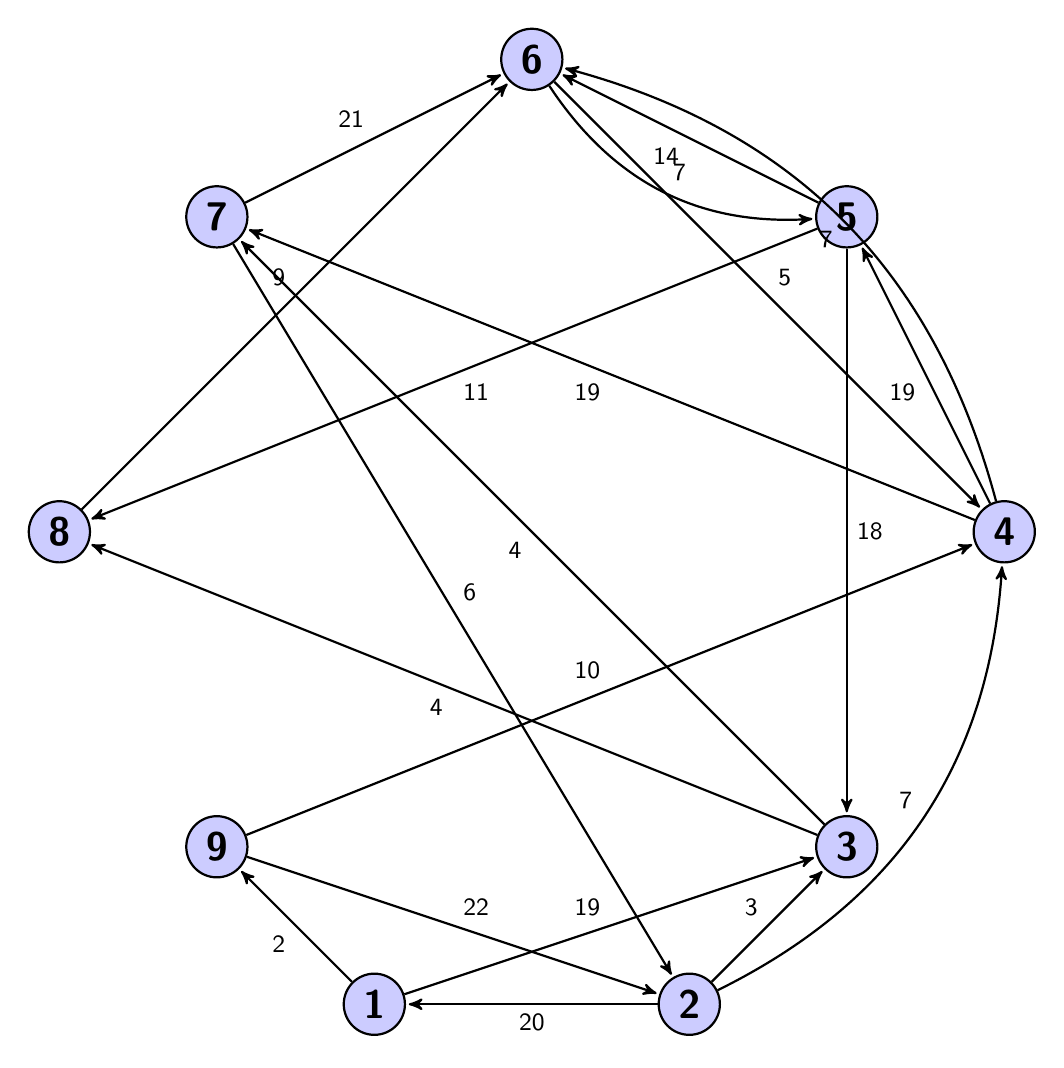
\begin{tikzpicture}[->,>=stealth',shorten >=1pt,auto,node distance=3cm,thick,main node/.style={circle,fill=blue!20,draw,font=\sffamily\Large\bfseries}]
  \node[main node] (1) at (10,0) {1};
  \node[main node] (2) at (14,0) {2};
  \node[main node] (3) at (16,2) {3};
  \node[main node] (4) at (18,6) {4};
  \node[main node] (5) at (16,10) {5};
  \node[main node] (6) at (12,12) {6};
  \node[main node] (7) at (8,10) {7};
  \node[main node] (8) at (6,6) {8};
  \node[main node] (9) at (8,2) {9};

\path[every node/.style={font=\sffamily\small}]
  (1) edge node {19} (3)
  (1) edge node {2} (9)
  (2) edge node {20} (1)
  (2) edge node {3} (3)
  (3) edge node {4} (7)
  (3) edge node {4} (8)
  (4) edge node {19} (5)
  (4) edge node {19} (7)
  (5) edge node {18} (3)
  (5) edge node {14} (6)
  (5) edge node {11} (8)
  (6) edge node {5} (4)
  (7) edge node {6} (2)
  (7) edge node {21} (6)
  (8) edge node {9} (6)
  (9) edge node {22} (2)
  (9) edge node {10} (4)
  (6) edge [bend right] node  {7} (5)
  (2) edge [bend right] node  {7} (4)
  (4) edge [bend right] node  {7} (6)
;
\end{tikzpicture}


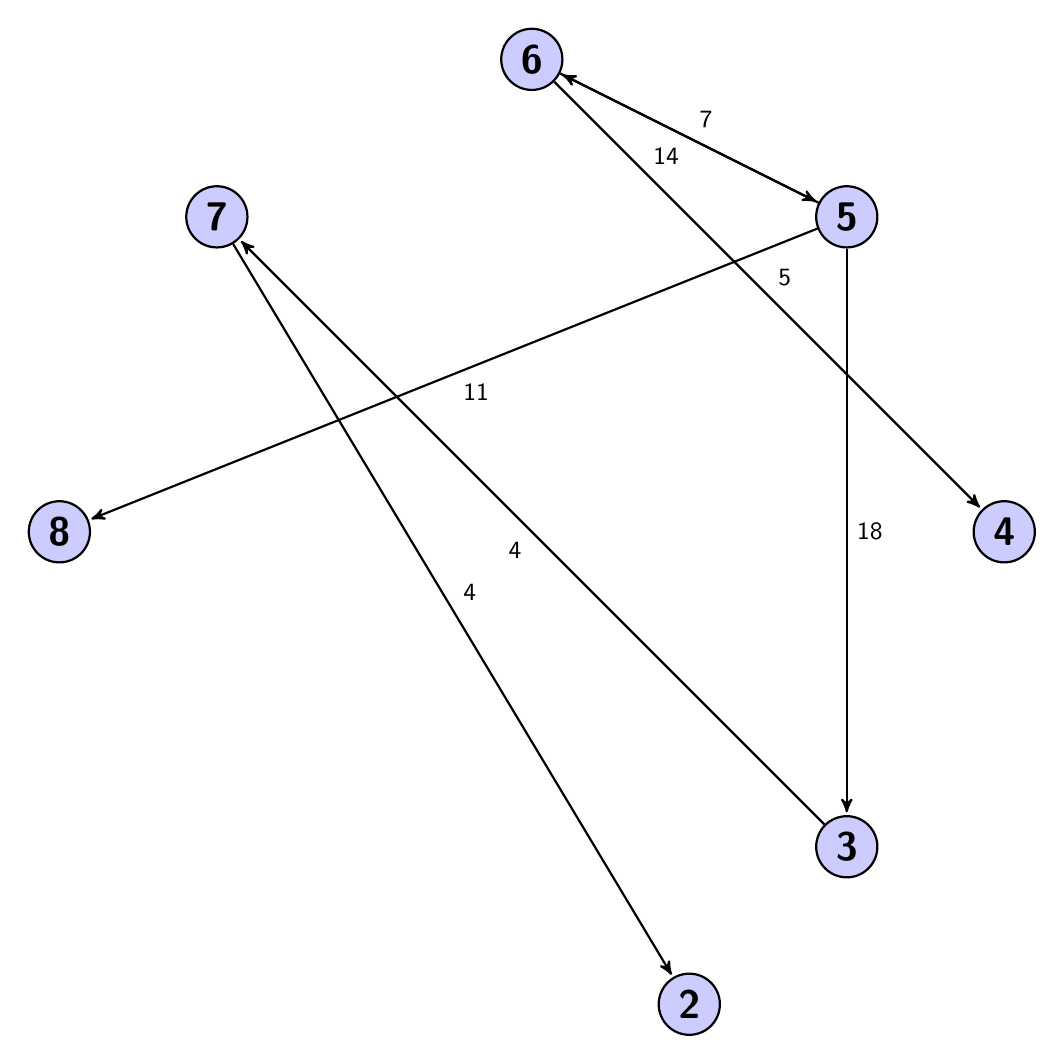
\begin{tikzpicture}[->,>=stealth',shorten >=1pt,auto,node distance=3cm,thick,main node/.style={circle,fill=blue!20,draw,font=\sffamily\Large\bfseries}]
  \node[main node] (2) at (14,0) {2};
  \node[main node] (3) at (16,2) {3};
  \node[main node] (4) at (18,6) {4};
  \node[main node] (5) at (16,10) {5};
  \node[main node] (6) at (12,12) {6};
  \node[main node] (7) at (8,10) {7};
  \node[main node] (8) at (6,6) {8};

\path[every node/.style={font=\sffamily\small}]
  (7) edge node {4} (2)
  (5) edge node {18} (3)
  (6) edge node {5} (4)
  (6) edge node {7} (5)
  (5) edge node {14} (6)
  (3) edge node {4} (7)
  (5) edge node {11} (8)
;
\end{tikzpicture}

\clearpage
path:5 3 7 2 
\\
capacity:4

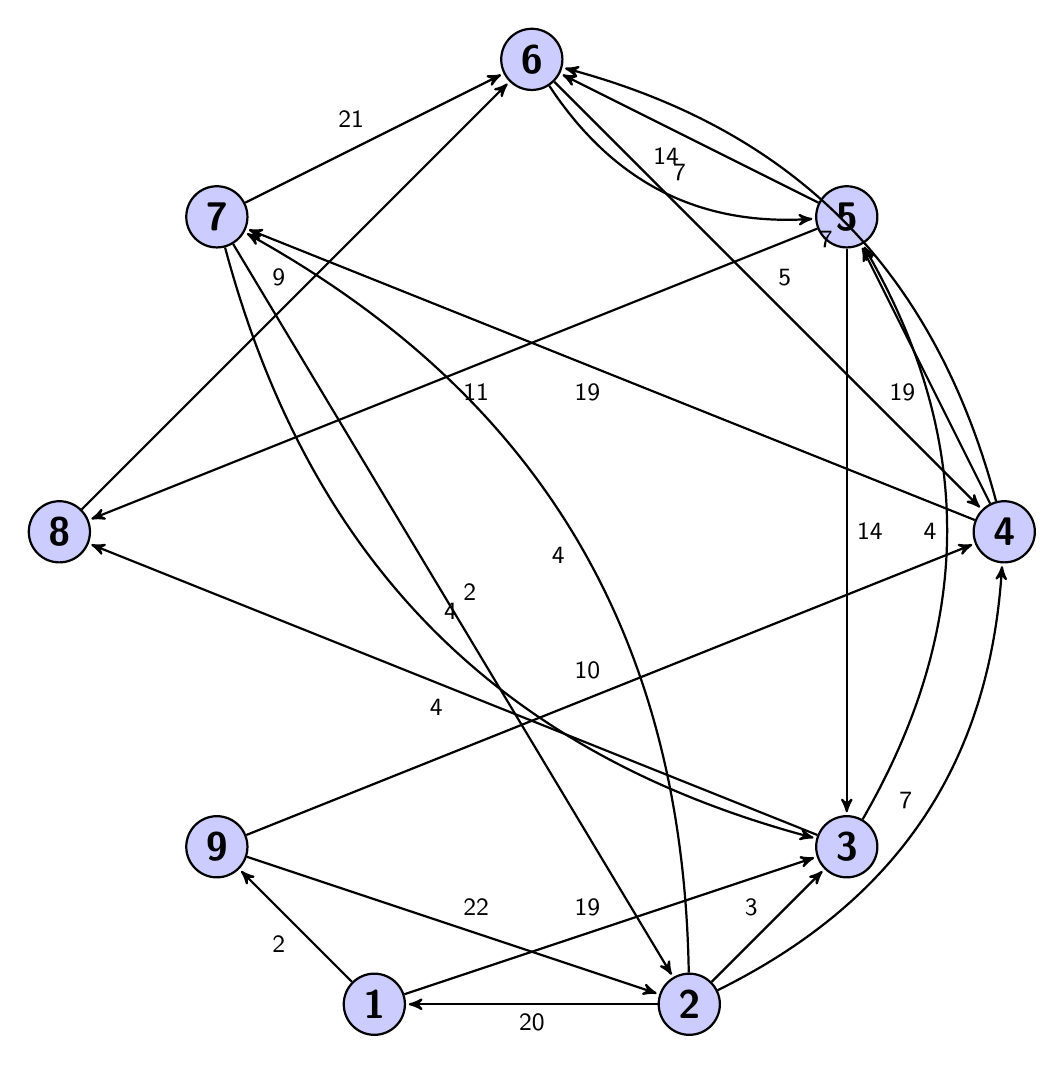
\begin{tikzpicture}[->,>=stealth',shorten >=1pt,auto,node distance=3cm,thick,main node/.style={circle,fill=blue!20,draw,font=\sffamily\Large\bfseries}]
  \node[main node] (1) at (10,0) {1};
  \node[main node] (2) at (14,0) {2};
  \node[main node] (3) at (16,2) {3};
  \node[main node] (4) at (18,6) {4};
  \node[main node] (5) at (16,10) {5};
  \node[main node] (6) at (12,12) {6};
  \node[main node] (7) at (8,10) {7};
  \node[main node] (8) at (6,6) {8};
  \node[main node] (9) at (8,2) {9};

\path[every node/.style={font=\sffamily\small}]
  (1) edge node {19} (3)
  (1) edge node {2} (9)
  (2) edge node {20} (1)
  (2) edge node {3} (3)
  (3) edge node {4} (8)
  (4) edge node {19} (5)
  (4) edge node {19} (7)
  (5) edge node {14} (3)
  (5) edge node {14} (6)
  (5) edge node {11} (8)
  (6) edge node {5} (4)
  (7) edge node {2} (2)
  (7) edge node {21} (6)
  (8) edge node {9} (6)
  (9) edge node {22} (2)
  (9) edge node {10} (4)
  (6) edge [bend right] node  {7} (5)
  (2) edge [bend right] node  {4} (7)
  (2) edge [bend right] node  {7} (4)
  (3) edge [bend right] node  {4} (5)
  (4) edge [bend right] node  {7} (6)
  (7) edge [bend right] node  {4} (3)
;
\end{tikzpicture}


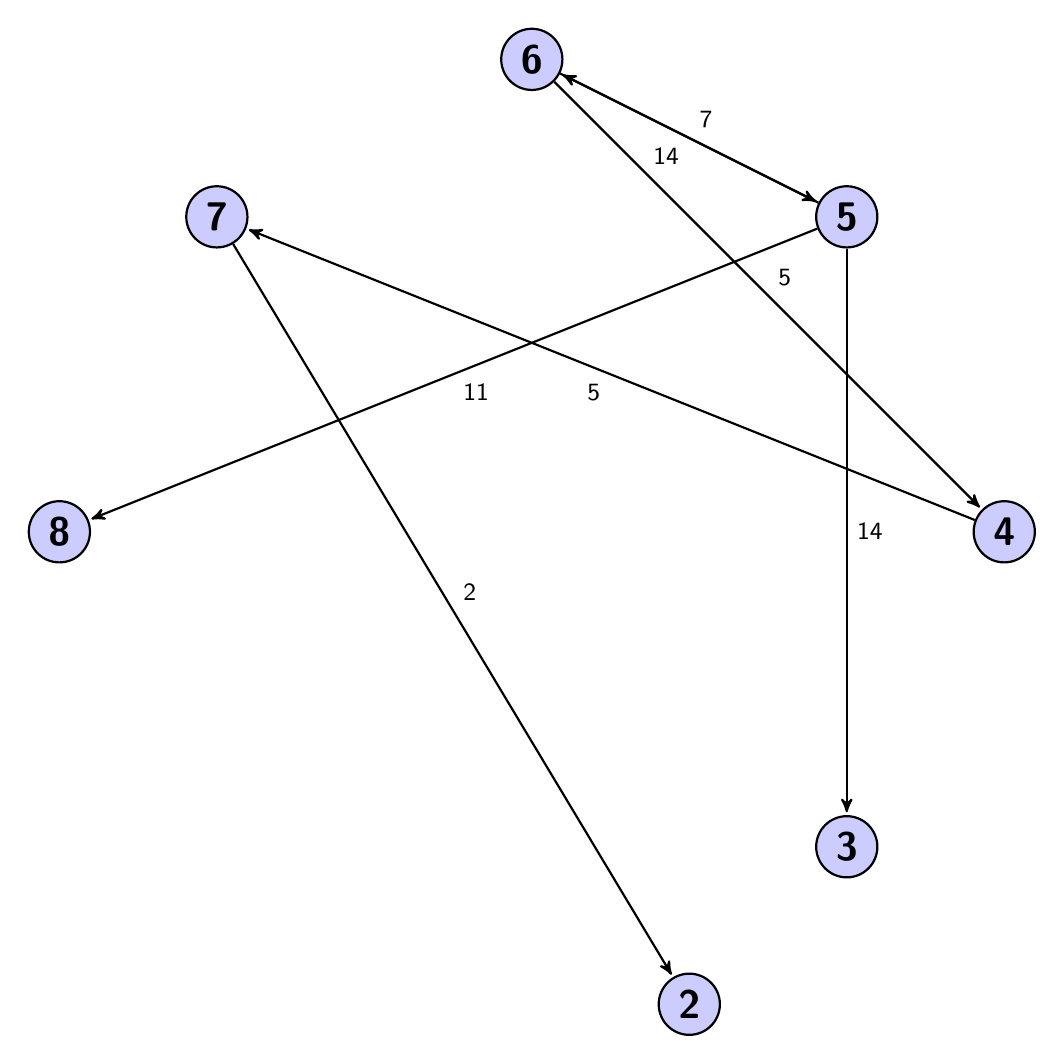
\begin{tikzpicture}[->,>=stealth',shorten >=1pt,auto,node distance=3cm,thick,main node/.style={circle,fill=blue!20,draw,font=\sffamily\Large\bfseries}]
  \node[main node] (2) at (14,0) {2};
  \node[main node] (3) at (16,2) {3};
  \node[main node] (4) at (18,6) {4};
  \node[main node] (5) at (16,10) {5};
  \node[main node] (6) at (12,12) {6};
  \node[main node] (7) at (8,10) {7};
  \node[main node] (8) at (6,6) {8};

\path[every node/.style={font=\sffamily\small}]
  (7) edge node {2} (2)
  (5) edge node {14} (3)
  (6) edge node {5} (4)
  (6) edge node {7} (5)
  (5) edge node {14} (6)
  (4) edge node {5} (7)
  (5) edge node {11} (8)
;
\end{tikzpicture}

\clearpage
path:5 6 4 7 2 
\\
capacity:2

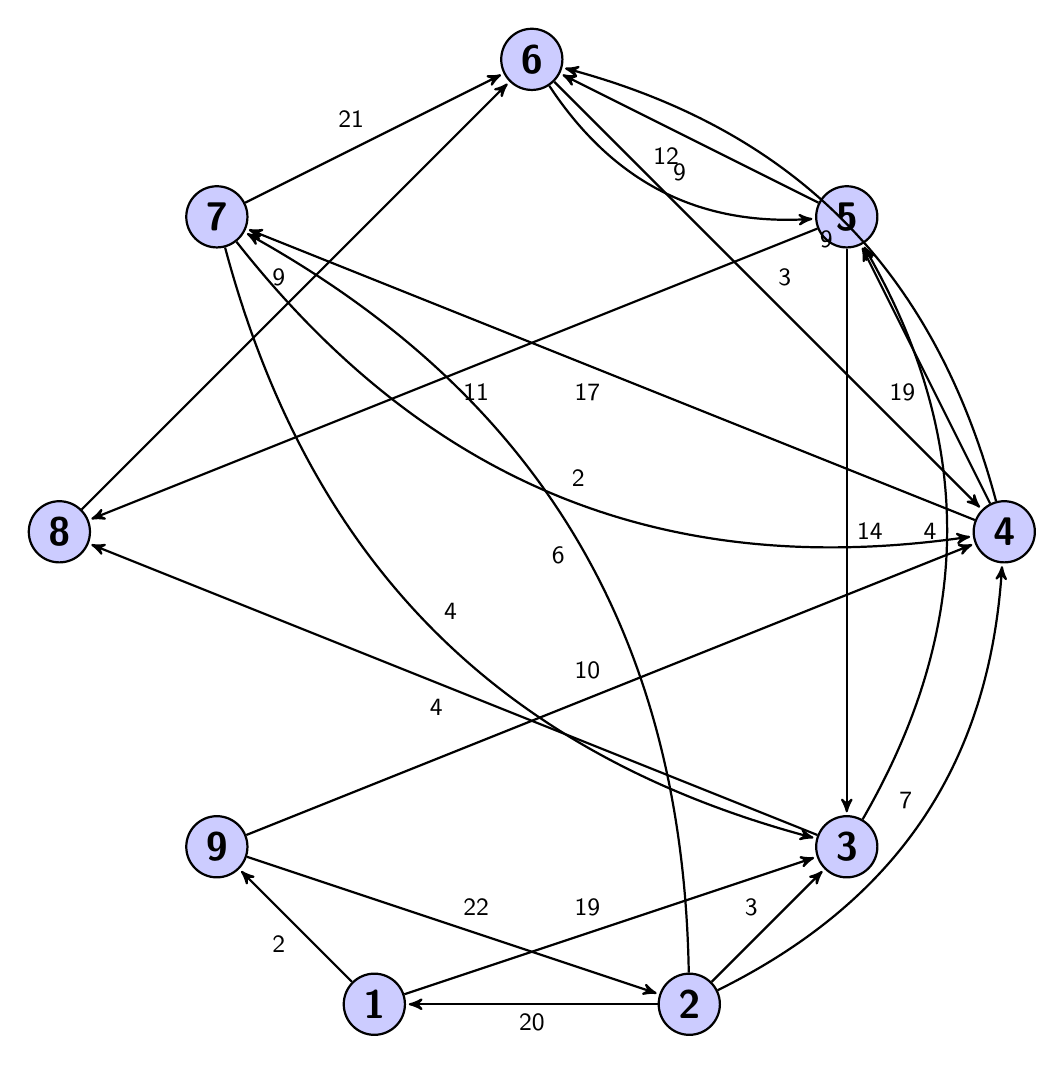
\begin{tikzpicture}[->,>=stealth',shorten >=1pt,auto,node distance=3cm,thick,main node/.style={circle,fill=blue!20,draw,font=\sffamily\Large\bfseries}]
  \node[main node] (1) at (10,0) {1};
  \node[main node] (2) at (14,0) {2};
  \node[main node] (3) at (16,2) {3};
  \node[main node] (4) at (18,6) {4};
  \node[main node] (5) at (16,10) {5};
  \node[main node] (6) at (12,12) {6};
  \node[main node] (7) at (8,10) {7};
  \node[main node] (8) at (6,6) {8};
  \node[main node] (9) at (8,2) {9};

\path[every node/.style={font=\sffamily\small}]
  (1) edge node {19} (3)
  (1) edge node {2} (9)
  (2) edge node {20} (1)
  (2) edge node {3} (3)
  (3) edge node {4} (8)
  (4) edge node {19} (5)
  (4) edge node {17} (7)
  (5) edge node {14} (3)
  (5) edge node {12} (6)
  (5) edge node {11} (8)
  (6) edge node {3} (4)
  (7) edge node {21} (6)
  (8) edge node {9} (6)
  (9) edge node {22} (2)
  (9) edge node {10} (4)
  (7) edge [bend right] node  {2} (4)
  (6) edge [bend right] node  {9} (5)
  (2) edge [bend right] node  {6} (7)
  (2) edge [bend right] node  {7} (4)
  (3) edge [bend right] node  {4} (5)
  (4) edge [bend right] node  {9} (6)
  (7) edge [bend right] node  {4} (3)
;
\end{tikzpicture}

13

%%%%%%%%%%%%%%%%%%%%%%%%%%%%%%%%%%%%%%%%%%%%%

\end{document}  